\begin{minipage}{0.50\textwidth}
    \begin{lstlisting}[style=CStyle]
#include <cstdint>

enum class CustomerType { 
    REGULAR, PREMIUM 
};

uint32_t 
processOrder(CustomerType customerType,
             uint32_t orderAmount,
             uint32_t loyaltyPoints,
             uint32_t specialEvent) 
{
  if (customerType == 
        CustomerType::REGULAR) {
    if (orderAmount > 100) {
      return orderAmount - 10;
    } else {
      return orderAmount;
    }
  else
    if (loyaltyPoints > 500) {
      return orderAmount - 10;
    } else {
      ++loyaltyPoints;
      return orderAmount;
    }
  }
}
    \end{lstlisting}
\end{minipage}%
\hspace{-1cm} % Adjust horizontal overlap
\begin{minipage}{0.40\textwidth}
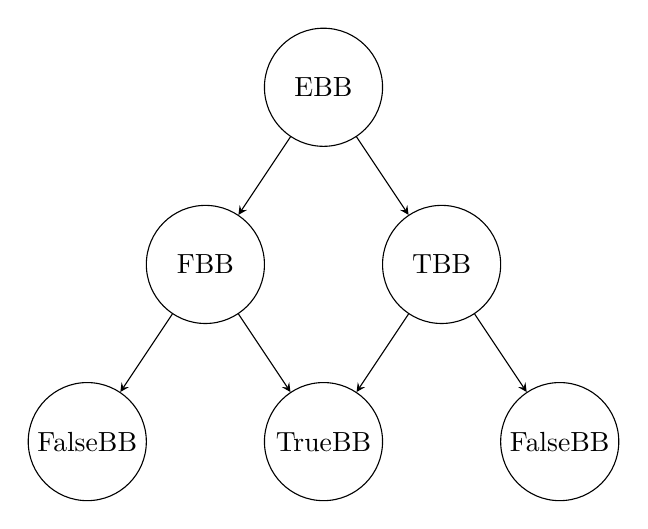
\begin{tikzpicture}[node distance=2cm and 3cm, >=stealth]
    % Style for consistent node dimensions
    \tikzstyle{node} = [circle, draw, fill=white, minimum size=1.5cm, inner sep=0]

    % Nodes
    \node[node] (EBB) at (1.5, 4.5) {EBB};
    \node[node] (TBB) at (3, 2.25) {TBB};
    \node[node] (FBB) at (0, 2.25) {FBB};
    \node[node] (TrueBB) at (1.5, 0) {TrueBB};
    \node[node] (FalseBB1) at (-1.5, 0) {FalseBB};
    \node[node] (FalseBB2) at (4.5, 0) {FalseBB};

    % Edges
    \draw[->] (EBB) -- (TBB);
    \draw[->] (EBB) -- (FBB);
    \draw[->] (TBB) -- (TrueBB);
    \draw[->] (TBB) -- (FalseBB2);
    \draw[->] (FBB) -- (TrueBB);
    \draw[->] (FBB) -- (FalseBB1);
\end{tikzpicture}
\end{minipage}